\subsection{Introduction to Decision Trees, Isolation Forest and Long Short-Term Memory}
This chapter provides a brief introduction to several machine learning models that are categorized as supervised learning models. These models are also the most relevant for the project.\\
The Decision-Tree-Classifier is one of the most well-known and powerful models in various fields. It works by creating a tree-like structure with nodes and branches, where each node represents an attribute or feature, and each branch represents the characteristic of the attribute \cite{decision_tree_explain}.
\begin{figure}[H]
  \centering
  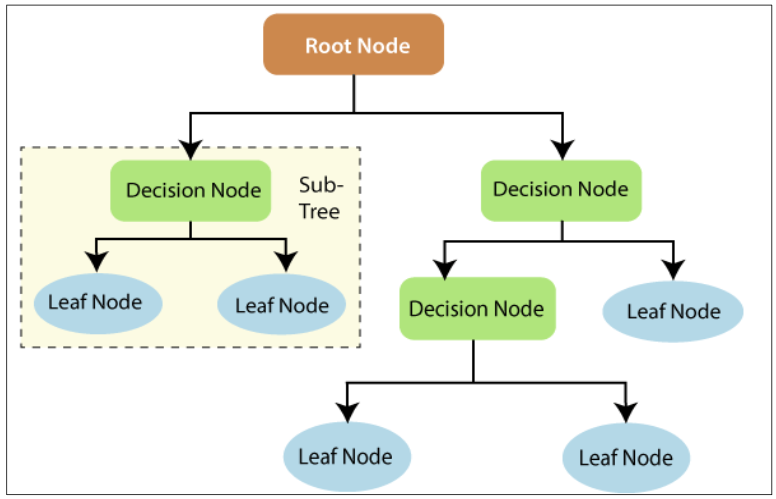
\includegraphics[width=0.5\textwidth]{pics/decision_tree_explain.png}
  \caption{Decision Tree \cite{decision_tree_explain}}
  \label{fig:decision_tree}
\end{figure}
The decision rule is not a black box and can be easily interpreted. It compares the value of the feature with a threshold and then decides which branch to follow. It is not only used in Machine Learning, but is also common in fields such as image processing and pattern recognition, due to its simple analysis and high accuracy. Despite these advantages, it has a high risk of overfitting, especially with small datasets \cite{decision_tree_explain}.\\

The \texttt{Random-Forest} is an ensemble method that combines multiple decision trees that work independently of each other. Each decision tree is created using a random vector to improve variance and reduce overfitting.\\
The final decision is made by a majority vote of all the trees together. This method is more robust against overfitting and can handle large datasets with high dimensionality. Two key factors influence the performance of the Random-Forest: the correlation between the trees and the strength of the individual trees \cite{breiman2001randomforests}.\\

The \texttt{Isolation-Forest} is an innovative approach for anomaly detection. While conventional methods typically create a model of "normal" behavior and classify deviations from it as anomalies, the Isolation-Forest follows the principle of directly isolating anomalies \cite{iForest}.\\
The explanation for this is that anomalies are characterized by their rarity and by being significantly different in their attributes. Therefore, they are easier to separate from the majority.\\
This model brings advantages such as robustness with regard to dimensionality and irrelevant features. On the other hand, swamping is one of the disadvantages, where normal instances that are too close to anomalies can prevent anomalies from being isolated and thus make them harder to detect \cite{iForest}.\\

A \texttt{Long Short-Term Memory (LSTM)} is a special type of Recurrent Neural Network (RNN) designed to model sequential data and long-term dependencies. Especially the long-term dependencies have high priority in this project, where the focus is on detecting anomalies across extended periods. LSTMs use memory cells and gating mechanisms to store information over long time steps reliably. Despite their many advantages, they come with many different parameters, making them difficult to tune. Additionally, they represent a black-box model, meaning it is hard to understand why the model made a certain decision \cite{LSTM_understanding}.

\begin{table}[H]
	\centering
	\begin{tabular}{|l|p{5cm}|p{5cm}|}
		\hline
		\textbf{Machine Learning Model} & \textbf{Advantages} & \textbf{Disadvantages} \\
		\hline
		Decision Tree & Easy to understand and interpret & High possibility of overfitting \\
		\hline
		Random-Forest & Less overfitting than a single decision tree; handles high-dimensional data & Not well-suited for small datasets \\
		\hline
		Isolation-Forest & Robust to high-dimensional and irrelevant features & Swamping effect in the presence of nearby normal instances \\
		\hline
		Long Short-Term Memory (LSTM) & Effective at modeling long-term dependencies & Black-box nature and complex parameter tuning \\
		\hline
	\end{tabular}
	\caption{Comparison of supervised learning models with advantages and disadvantages \cite{decision_tree_explain}\cite{breiman2001randomforests}\cite{iForest}\cite{LSTM_understanding}.}
    \label{tab:supervised_learning_models}
\end{table}